
\section{Introduction}
The introduction of hardware HEVC encoders to consumer-grade GPUs has opened the door to mass 360-degree and 4K video livestreaming, but does not immediately offer a solution to adaptive video streaming. Recently, a significant body of work on tile-based adaptive streaming for 360-degree and 4K video has appeared, in which the quality requested for each section of a video corresponds to how interesting it is, allowing clients to view the most important parts of a video, or, e.g., those which a user is moving their head towards, in high-quality without stalling. This is straightforward for pre-rendered video, but is more complicated in a livestreaming scenario because each quality requires another encode, necessarily introducing some delay in the availability of a new segment. Furthermore, tiling, which must occur within the HEVC encoder prior to generation of the bitstream, is not supported by existing hardware encoders. One can try to get around this by feeding each tile to the encoder as a separate video and stitching them together afterwards, but even top-of-the-line consumer-grade GPUs only support two contiguous encoding processing, forcing the user to either encode the whole frame at two different qualities, or divide each frame into two tiles but only offer a single quality for either tile. In the former case, tiling does not occur; in the latter, the tile sizes are so large as to render the point moot, and the video stream is not adaptive because only one quality is available for either half.

To combat these challenges, we introduce RATS, a GPU-based HEVC encoding pipeline to tile, encode, and stitch video at multiple qualities in real-time on a frame-by-frame basis. RATS uses HEVC slices in conjunction with tiles to encode each region of a video independently, so that a player can pick and choose which quality they want for each region. To do so, the source video stream is divided into vertical strips, which are stacked on top of one another. This rearranged video image is fed to the encoder with slice boundaries specified to at least be the edges of these strips, so that each slice is some fraction of the horizontal width and, possibly, vertical height. This process occurs twice for each frame with different bitrate configurations, resulting in high-quality and low-quality outputs. When the video is reconstructed during playback, each slice is an independently-decodable region of video, so we are free to pick and choose either quality for each region of the video shown to the user.

The rest of this paper is organized as follows: ...


\begin{figure*}[t]
	\centering
	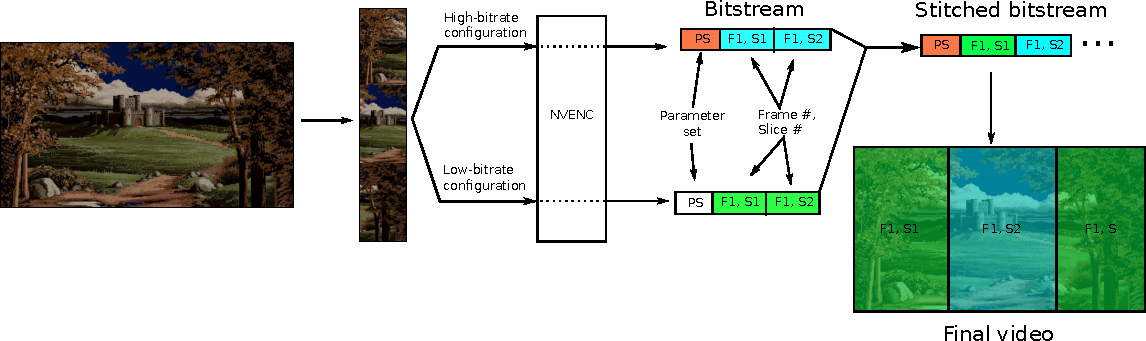
\includegraphics[width=\textwidth]{figures/pipeline.pdf}
	\caption{An illustration of the pipeline}
\end{figure*}

\section{HEVC and NVENC}

The most computation-heavy components of the HEVC encoding process, such as motion estimation, are not easily parallelized. Parallel HEVC video encoding instead relies on dividing each frame of the video into independent regions, encoding them separately, and joining their edges during playback. Two versions of this concept, slices and tiles, exist within the HEVC standard. Functionally, they are identical; however, slices are limited to chunking the video into wide strips, while tiles can divide a video into rectangular CTU-based areas of any size. While tiles are supported by most decoders, very few encoders allow for it, all of which are software encoders far too slow to operate in real-time. 

HEVC encoders convert raw video into an HEVC bitstream consisting of multiple sequential NAL units via a complex implicit syntax. Each NAL unit contains some header information followed by raw image data. For videos without slicing or tiling, most NAL units correspond to a single full frame of video; however, because slices and tiles are independently-decodable, each tile or slice within a video frame is a self-contained NAL unit. Interestingly, we can then treat any rectangular arrangement of HEVC bitstreams as tiles within a single video by alternating their NAL units and manipulating specific values in the NAL headers. This process, in which multiple bitstreams are joined to form one bitstream which displays all constituent bitstreams in different regions of the final video, is known as \textit{stitching}. (Maybe include some references to works which do stitching or something)

NVENC is a hardware video encoder present on newer Nvidia GPUs, and is the state-of-the-art hardware HEVC encoder. Note that HEVC is not easily data-parallelizable; as a result, NVENC is an ASIC separate from the CUDA cores. Interaction with NVENC occurs via the NVENCODE API, and offers the user a handful of parameters for the encoder, such as target bitrate, slice boundaries, and GOP specifications. It is possible to swap out encoder configurations between frames, allowing one to encode multiple videos simultaneously, but even top-of-the-line consumer GPUs only support a maximum of two contiguous configurations. Note that these configurations are not simply encoding parameters, but also contain, e.g., the previous frame data necessary to encode the next P- or B-frame. This is a limitation enforced by the driver, and supercomputing GPUs, such as the Nvidia Titan V, do not have such limits. Such GPUs are, however, prohibitively expensive for most consumers, so we do not consider them here.

\section{RATS Implementation}
To work within the confines imposed by NVENC, namely the lack of tile support and limitation to two simultaneous encoding sessions, we divide the real-time adaptive encoding pipeline into an encoding component, in which a raw video frame is manipulated and converted into low- and high-quality bitstreams, and a stitching component, in which these bitstreams are combined to be displayed to the user.

\subsection{Encoding}
NVENC supports multiple slice modes, one of which, \texttt{sliceMode=3}, cuts the video into $n$ equal slices as specified via the \texttt{sliceModeData=}$n$ parameter. Vertical cuts, which are important for 360-degree video, cannot be made via slices, but the image boundaries are natural slice boundaries as well. We therefore manipulate the input images by vertically cutting them into $n$ pieces of equal size and stacking these pieces on top of each other, then setting \texttt{sliceModeData=}$n$, so that the slice boundaries align with the top and bottom boundaries of the original image. The output bitstream from the encoder will then typically contain $n+1$ NAL units per frame, one for each slice and a single SEI at the end. During the stitching process, specific changes will be made to the NAL headers to instead treat these slices as tiles and place them side-by-side in the final video bistream.

In a YUV420p video, each frame of the video consists of the titular Y, U, and V components, corresponding to the luminance and two chrominance components, respectively. These components are laid out sequentially as well, such that the luminance of the image is described, then one chrominance component, then the other. Each byte within the luminance component corresponds to a single pixel in the image, but each byte within a chrominance component corresponds to a $2\times2$ pixel area. Either chrominance component is therefore a quarter of the size of the luminance component. 

Rearranging is performed on each component via memcpy, with a length equal to the width of a tile column. Recall that the purpose of rearranging is to set the vertical tile boundaries, as NVENC slicing will handle the horizontal tile boundaries. Tile rows are therefore ignored at this stage. Within each tile column, we begin at the first pixel row and move down, calling memcpy on each pixel row and placing the contents in a new array, before moving on to the next tile column once we hit the bottom of the image. The result of this process will be an image in which the tile columns are effectively stacked on top of one another.

To interact with NVENC, we use the libavcodec API provided by FFmpeg. This API handles much of the tedium of using NVENC, allowing us to simply do some initialization and call a handful of methods to interact with the GPU. The high- and low-bitrate configurations are distinct instances of the AVCodecContext struct, which are initialized before the encoding process begins. During the encoding process, a rearranged image is passed to NVENC twice, once with each AVCodecContext instance, to obtain the low- and high-bitrate bitstreams. Within NVENC, we set sliceModeData equal to the total number of tiles desired. The left and right tile boundaries will be the edges of the image fed to NVENC, so the slicing will create the top and bottom boundaries.

\subsection{Stitching}
The bitstreams resulting from the encoding process contain the independently-decodable slices which will function as our tiles, but they will still be stacked from top-to-bottom. Fortunately, we must only modify a few fields in the NAL headers to convert the slices to tiles and arrange them in the desired configuration. Table ~\ref{tab:stitch} lists all such fields. Note that within an HEVC bitstream, \textit{NAL} and \textit{slice} are equivalent terms which may be used interchangeably. To avoid confusion, we will retain the use of "slice" to refer to an independently-decodable horizontal strip of an image.

In addition to modifying those values listed in Table ~\ref{tab:stitch}, there are two more changes necessary on behalf of emulation prevention bytes and byte alignment. NAL borders are represented by the byte-aligned sequence \texttt{0x000001}. To prevent this sequence from occurring by chance within a NAL, the byte-aligned sequence \texttt{0x03}, referred to as the emulation prevention byte, may be inserted after any \texttt{0x0000} which is not part of a NAL border. The emulation prevention byte has no other meaning and does not otherwise impact the NAL parsing process. 

If the stitching process modifies the number of bits in the NAL header by, e.g., inserting a new field or changing the value of an unsigned Exponential Golomb code, any emulation prevention bytes appearing after the point of change will likely cease to be byte-aligned. The decoder will then consider these bits to have semantic value, resulting in a corrupt or incorrect header. We must also ensure that the stitching process does not introduce any new \texttt{0x0000} sequences without a trailing emulation prevention byte. To tackle both of these issues at once, we discard any emulation prevention bytes we encounter in the original NAL and check for any \texttt{0x0000} sequences after our changes have been made. No such concern is necessary for the NAL data because this data will be byte-aligned at the end of the header.

Byte alignment occurs at the end of a NAL header or NAL data. After the last semantic bit, a \texttt{1} is appended to the NAL section, followed by as many \texttt{0}s as necessary to complete the byte. As is the case with emulation prevention bytes, if the size of the NAL header changes during modification, we will likely have an incorrect number of trailing \texttt{0}s. To redo the byte alignment, we find the last \texttt{1} in the original NAL and remove it and everything after it, effectively undoing the previous byte alignment. We then perform byte alignment after our modifications have been made.

The stitching process is performed with the Boost C++ dynamic\_bitstream API, which allows one to read bytes into a vector of bits, manipulate these bits, then convert the bit vector into raw bytes. The high- and low-bitrate configurations are identical except for the specified bitrate, and the resulting NAL headers do not change based on, e.g., content, so the output from NVENC is highly predictable. Therefore, navigating to the right spot in the bitstream and making our changes is a straightforward process.

\renewcommand{\figurename}{Tab.}
\setcounter{figure}{1}
\begin{table*}[t]
	\centering
	\begin{tabular}{llp{3in}r}
		\toprule
		NAL Type & Field & Description & Fixed value \\
		\midrule
		\multirow{2}{*}{SPS} & \texttt{pic\_width\_in\_luma\_samples} & Pixel width of the final video. & \\ \cmidrule[0.5pt]{2-4}
		& \texttt{pic\_hidth\_in\_luma\_samples} & Pixel height of the final video. & \\
		\midrule[1pt]
		\multirow{5}{*}[-5em]{PPS} & \texttt{tiles\_enabled\_flag} & Converts slices to tiles and adds several relevant fields to the bitstream syntax. & \texttt{1} \\ \cmidrule[0.5pt]{2-4}
		& \texttt{num\_tile\_columns\_minus1} & Number of tile colums minus 1. & \\ \cmidrule[0.5pt]{2-4}
		& \texttt{num\_tile\_rows\_minus1} & Number of tile rows minus 1. & \\ \cmidrule[0.5pt]{2-4}
		& \texttt{uniform\_spacing\_flag} & Whether tiles are evenly sized. If \texttt{0}, manual tile boundaries must be specified. & \texttt{1} \\ \cmidrule[0.5pt]{2-4}
		& \texttt{loop\_filter\_across\_tiles\_enabled\_flag} & Whether in-loop filtering should be performed across tile boundaries. This is optional, and may be desired if there is less of a difference between the high and low bitrates. & \texttt{1} \\
		\midrule[1pt]
		\multirow{4}{*}[-6em]{\shortstack{I-slice, \\P-slice}} & \texttt{first\_slice\_segment\_in\_pic\_flag} & Should be \texttt{1} in the top-leftmost tile, and \texttt{0} in all other tiles. If \texttt{0}, the slice segment address must be specified. & \\ \cmidrule[0.5pt]{2-4}
		& \texttt{slice\_segment\_address} & The address of the top-leftmost CTU in this tile, beginning from 0 at the top-leftmost CTU in the entire image, and incrementing across the image, moving down and continuing at the end of the row.& \\ \cmidrule[0.5pt]{2-4}
		& \texttt{slice\_loop\_filter\_across\_slices\_enabled\_flag} & Similar to the loop filter flag in the PPS, but specifically concerned with in-loop filtering across the left and top boundaries of the tile. & \texttt{1} \\ \cmidrule[0.5pt]{2-4}
		& \texttt{num\_entry\_point\_offsets} & Used to treat \texttt{emulation\_prevention\_three\_byte} as part of the tile data, which is not desired here. & \texttt{1} \\
		\bottomrule
	\end{tabular}
	\caption{Table containing all NAL header modifications. The "Fixed value" column contains the bit values of hard-coded fields, such as important flags. Missing values indicate that the value may vary depending on the video and parameters used. In this case, all such values would be encoded using unsigned Expontential-Golomb.}
	\label{tab:stitch}
\end{table*}
\renewcommand{\figurename}{Fig.}
\setcounter{figure}{2}

\section{Installing and Using RATS}
RATS was developed and evaluated on Ubuntu 18.04, using CUDA 9.2, FFmpeg 3.4, and Boost 1.64. We use a slightly modified version of FFmpeg which sets \texttt{sliceModeData=3} and adds a new field, \texttt{numSlices}, to \texttt{AVCodecContext} so that we may specify the tile configuration at run-time. FFmpeg must be configured with CUDA support, and to produce static libraries.

To build RATS, first clone the git repository \textbf{https://github.com/\\ballardt/nvenc-live}. Modify the paths in \texttt{build.sh} to point to the FFmpeg static libraries, then run it. The resulting executable, \texttt{encode}, is the RATS command-line program.

More details on installation and usage can be found in the git repository.

\section{Evaluation}
To evaluate RATS, we compare its performance to an existing tiling video encoder, investigate the impact on tile size and quality on performance, and measure the relative time of the rearranging, encoding, and stitching components.

To the best of our knowledge, RATS contains the first available HEVC tile stitcher. Furthermore, RATS is the first GPU-powered tile-based encoder. It is therefore difficult to directly compare RATS to other programs; software-based tiling encoders will clearly be much slower and cannot be stitched, and GPU encoders without RATS simply perform one step of the RATS pipeline without the others. However, it is worthwhile to have some idea of how much more quickly this work is than existing software encoders. 

\begin{figure}[t]
	% \includegraphics[width=\columnwidth]{figures/hevc_eval_qual.png}
	\caption{Encoding speed vs. tile quality for $4\times4$ tiles. All tiles on the left are of the high bitrate, while those on the right are of the low bitrate.}
\end{figure}

\begin{figure}[t]
	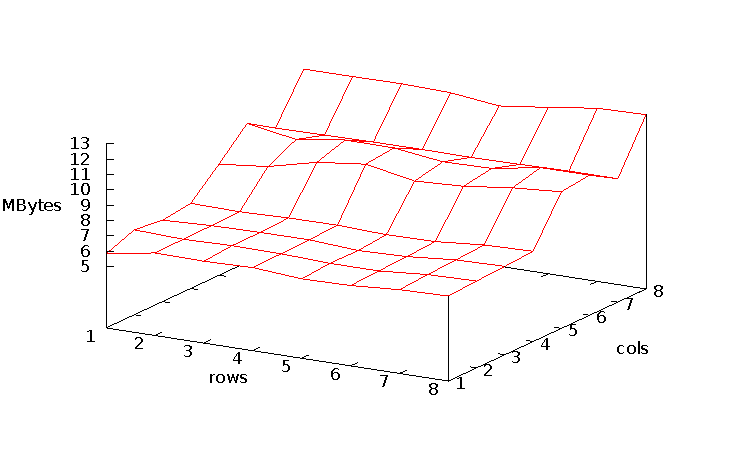
\includegraphics[width=\columnwidth]{figures/Sizes.pdf}
	\caption{Encoding output size across tile configurations. In each case, half of the tiles are of a high bitrate, half are of a low bitrate, and tile qualities alternate in a checkerboard pattern.}
\end{figure}

\begin{figure}[t]
	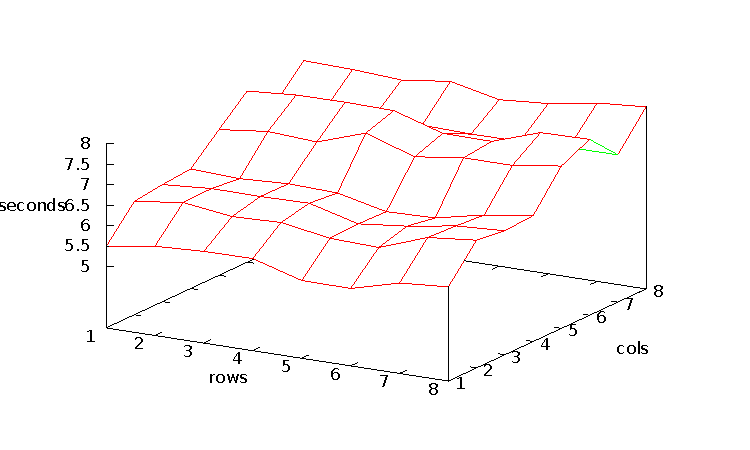
\includegraphics[width=\columnwidth]{figures/Times.pdf}
	\caption{Encoding speed across tile configurations. The tile qualities alternate between high and low in a checkerboard pattern. Each configuration has an odd number of tiles, and we set the extra tile to be low quality. The video used was 30s long, so the red line indicates the speed necessary to achieve real-time ABR encoding.}
\end{figure}


\section{Conclusion}

\section{Notes, to be deleted}
Sharing CUDA contexts (not used): https://devtalk.nvidia.com/default/topic/1031189/video-codec-sdk/sharing-the-same-cuda-context-for-encoding-nvenc-and-decoding-nvdec-/

NVIDIA patch (used): https://github.com/keylase/nvidia-patch
